\uuid{49BI}
\exo7id{7153}
\titre{exo7 7153}
\auteur{megy}
\organisation{exo7}
\datecreate{2017-05-13}
\isIndication{true}
\isCorrection{true}
\chapitre{Géométrie affine euclidienne}
\sousChapitre{Géométrie affine euclidienne du plan}
\module{Géométrie}
\niveau{L2}
\difficulte{}

\contenu{
\texte{
Soit $ABC$ un triangle rectangle en $A$ et non isocèle. La médiatrice de $[BC]$ recoupe le demi-cercle circonscrit en $I$. On considère deux points $D\in [AB]$ et $E \in [AC]$ tels que $BD=CE$. Montrer que $IDE$ est rectangle isocèle en $I$.

\begin{center}
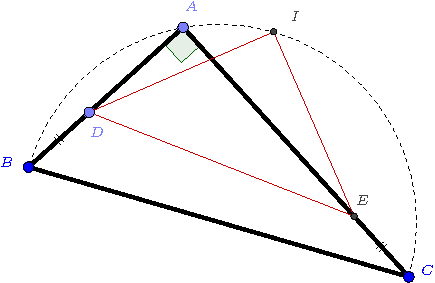
\includegraphics{../images/49BI-1}
\end{center}
}
\indication{Considérer la similitude directe qui envoie le couple $(B,D)$ sur le couple $(C,E)$.}
\reponse{
Il existe une unique similitude directe qui envoie le couple $(B,D)$ sur le couple $(C,E)$. Comme $BD=CE$, c'est une isométrie donc une rotation, et comme $(\overrightarrow{BD},\overrightarrow{CE}) = \pi/2$, son angle est $\pi/2$.

Or, il n'y a qu'une rotation d'angle $\pi/2$ qui envoie $B$ sur $C$ : son centre est $I$. On en déduit que $IDE$ est rectangle isocèle en $I$.
}
}
